\chapter{Rings and Ideals}

Let $R$ be a CRW1.

\begin{fact}
    $R = 0$ iff $1_R = 0_R$.
\end{fact}

\begin{fact}
    \begin{enumerate}[(1)]
        \item $1_R$ and $0_R$ are both unique.
        \item For any $r \in R$, $-r$ is unique.
        \item If $r \in R$ is a unit, i.e., there exists $r^{-1} \in R$ such that $rr^{-1} = 1_R = r^{-1}r$, then $r^{-1}$ is also unique.
    \end{enumerate}
\end{fact}

\begin{definition}
    A homomorphism of CRW1's is a function $\phi: R \to S$, where $R$ and $S$ are CRW1's, such that 
    \begin{enumerate}[(1)]
        \item $\phi(r+r') = \phi(r) + \phi(r')$,
        \item $\phi(rr') = \phi(r) \phi(r')$,
        \item $\phi(1_R) = 1_S$.
    \end{enumerate}
    A.K.A. a ring homomorphism.
\end{definition}

\begin{fact}
    Let $\phi: R \to S$ be a ring homomorphism.
    \begin{enumerate}[(a)]
        \item $\phi(0_R) = 0_S$.
        \item $\phi(-r) = -\phi(r)$ for any $r \in R$.
        \item $\phi(r-s) = \phi(r) - \phi(s)$ for any $r,s \in R$.
        \item $\phi(\sum_{i=1}^mr_is_i) = \sum_{i=1}^m\phi(r_i)\phi(s_i)$ for any $r_1,\cdots,r_m,s_1,\cdots,s_m \in R$.
        \item If $r$ is a unit in $R$, then $\phi(r)$ is a unit in $S$ and $\phi(r)^{-1} = \phi(r^{-1})$.
        \item A composition of ring homomorphisms is a ring homomorphism.
    \end{enumerate}
\end{fact}

\begin{definition}
    A \emph{subring} of $R$ is a subset $S \subseteq R$ such that $S$ is a CRW1 under the operations for $R$ and such that $1_S = 1_R$, i.e., $1_R \in S$.
\end{definition}

\begin{fact}[Subring test]
    A subset $S \subseteq R$ is a subring iff it is closed under $+,\cdot,-$ and $1_R \in S$.
\end{fact}

\begin{example}
    Subring test: need $\emptyset \neq S \subseteq R$, $S$ is closed under $+,\cdot,-$ and $1_R \in S$. \\
    If $S$ is not closed under $-$, then fail. Let $\bbN_0 = \{0,1,2,\cdots\} \subseteq \bbZ$ not a subring. \\
    If $1_R \not \in S$, then fail. $R = \bbF_3 \times \bbF_3 \supseteq \{(a,a) \mid a \in \bbF_3\} =: S$. Then $S$ is a subring of $R$. Although $S_1 := \{(a,0) \mid a \in \bbF_3\} \cong \bbF_3 \cong \{(0,a) \mid a \in \bbF_3\} =: S_2$ are rings but not subrings of $R$ since $1_R = (1,1) \not \in S_1$ and $1_R = (1,1) \not \in S_2$. 
\end{example}

\begin{fact}
    If $S \subseteq R$ is a subring, then the inclusion map $\varepsilon: S \to R$ given by $\varepsilon(s) = s$ is a ring homomorphism.
\end{fact}

\begin{definition}
    An \emph{ideal} of $R$ is a non-empty subset $\ffa \subseteq R$ and a subgroup under addition such that for any $r \in R$ and any $a \in \ffa$, $ra \in \ffa$. \\
    An ideal $\ffa \leq R$ is \emph{prime} if $\ffa \neq R$ and for any $a,b \in R$, if $a,b \not \in \ffa$, then $ab \not \in \ffa$, i.e., if $ab \in \ffa$, then $a \in \ffa$ or $b \in \ffa$. \\
    An ideal $\ffa \leq R$ is \emph{maximal} if $\ffa \neq R$ and for any ideal $\ffb \leq R$, if $\ffa \subseteq \ffb \subseteq R$, then either $\ffa = \ffb$ or $\ffb = R$.
\end{definition}

\begin{fact}[Ideal test]
    If $\ffa \neq \emptyset$ and $\ffa$ is closed under $\cdot$, then for any $a \in \ffa$, $-a = (-1_R)a \in \ffa$, also, since $\ffa$ is closed under $+$, it is automatically closed under $-$. \\
    Thus, A subset $\ffa \subseteq R$ is an ideal iff $\ffa \neq \emptyset$ and $\ffa$ is closed under $+$ and $\cdot$. 
\end{fact}

\begin{example}
    \begin{enumerate}[(a)]
        \item 
            Let $R = \bbZ$, then ideals of $R$ are $n\bbZ = \{nm \mid m \in \bbZ\}$, where $n \in \bbZ$. \\
            $n\bbZ$ is prime iff $n = 0$ or $\abs n$ is prime. \\
            $n\bbZ$ is maximal iff $\abs n$ is prime.
        \item 
            If $I_\lambda \leq R$ for any $\lambda \in \Lambda$, then $\bigcap_{\lambda \in \Lambda} I_\lambda \leq R$.
        \item 
            If $r_1,\cdots,r_m \in R$, then 
            \begin{align*}
                \langle r_1,\cdots,r_m \rangle &= \langle r_1,\cdots,r_m \rangle R = (r_1,\cdots,r_m) = (r_1,\cdots,r_m)R = \bigcap_{r_1,\cdots,r_m \in I \leq R} I \\
                                               &= \left\{\sum_{i=1}^m a_ir_i \mathrel{\bigg |} a_i \in R,\fa i = 1,\cdots,m\right\} \leq R. 
            \end{align*}
            In particular, for any $r \in R$, $\langle r \rangle = \langle r \rangle R = (r) = (r)R = rR = Rr = \{ar \mid a \in R\} = \bigcap_{r \in I \leq R}I$.
        \item 
            If $A \subseteq R$, then $\langle A \rangle = \bigcap_{A \subseteq I \leq R}I$ and $\langle A \rangle = \{\sum_{a \in A}^{\text{finite}} r_a a \mid r_a \in R,\fa a\}$.
    \end{enumerate}
\end{example}

\begin{fact}
    For any $r_1,\cdots,r_m \in R$, $\langle r_1,\cdots,r_m \rangle$ is the smallest ideal of $R$ containing $r_1,\cdots,r_m$, i.e., for any $\ffa \leq R$, $r_1,\cdots,r_m \in \ffa$ iff $\langle r_1,\cdots,r_m \rangle \subseteq \ffa$. Similarly, $A \subseteq \ffa$ iff $\langle A \rangle \subseteq \ffa$. For example, if $A \leq R$, then $A = \langle A \rangle$.
\end{fact}

\begin{construction}
    Let $\ffa \leq R$. For any $r \in R$, $r+\ffa = \{r + a \mid a \in \ffa\} = \overbar r$. Let $R/\ffa := \{r + \ffa \mid r \in R\}$. Then $R/\ffa$ is a CRW1 with $\overbar r \pm \overbar s = \overbar {r \pm s}$, $\overbar r \overbar s = \overbar{rs}$, $0_{R/\ffa} = \overbar {0_R}$ and $1_{R/\ffa} = \overbar {1_R}$. \\
    Let $\pi: R \to R/\ffa$ be given by $\pi(r) = \overbar r$. Then $\pi$ is a well-defined ring epimorphism.
    \begin{center}
        \begin{tikzcd}
            R \arrow[r,"\phi"] \arrow[d,"\pi"] & S \\
            R/\ffa \arrow[ru,dashed,"\ex !\ \overbar \phi"']
        \end{tikzcd}
    \end{center}
    For any $\phi: R \to S$ ring homomorphism, if $\phi(\ffa) = 0$, then there exists a unique ring homomorphism $\overbar \phi: R/\ffa \to S$ making the diagram commute, where $\overbar \phi(\overbar r) = \overbar \phi (\pi(r)) = \phi(r)$. \\
    Note $\phi(\ffa) = 0$ iff $\ffa \subseteq \ker(\phi)$. In particular, if $\ffa = \langle A \rangle$, then $\ffa \subseteq \ker(\phi)$ iff $A \subseteq \ker(\phi)$.
\end{construction}

\begin{fact}
    Let $\ffa \leq R$. 
    \begin{enumerate}[(a)]
        \item $\ffa$ is prime iff $R/\ffa$ is an integral domain.
        \item $\ffa$ is maximal iff $R/\ffa$ is a field.
        \item If $R$ is a field, then it is an integral domain. So if $\ffa$ is maximal, then $\ffa$ is prime.
    \end{enumerate}
\end{fact}

\begin{fact}[Ideal correspondence for quotients]
    Let $\ffa \leq R$ and $\pi: R \to R/\ffa$ be the canonical epimorphism. 
    \begin{align*}
        \{\text{ideals }I \leq R/\ffa\} &\rightleftarrows \{\text{ideals }J \leq R \mid \ffa \subseteq J\} \\
        I &\mapsto \pi^{-1}(I) = \{r \in R \mid r + \ffa \in I\} \\
        J/\ffa &\mapsfrom J \\
    \{\text{ideals } I \leq R/\ffa\} &\rightleftarrows \{\text{ideals }J \leq R \mid \ffa \subseteq J\} \\
        \{\text{primes ideals of } R/\ffa\} &\rightleftarrows \{\text{prime ideals }\ffp \leq R \mid \ffa \subseteq \ffp\} \\
        \{\text{maximal ideals of } R/\ffa\} &\rightleftarrows \{\text{maximal ideals }\ffm \leq R \mid \ffa \subseteq \ffm\}
    \end{align*}
    In both $R$ and $R/\ffa$, maximal ideals are a subset of prime ideals and prime ideals are a proper subset of ideals. \\
    Claim $\frac{R/\ffa}{J/\ffa} \cong \frac{R}{J}$.
    \begin{center}
        \begin{tikzcd}
            R \arrow[d,two heads,"\pi"] \arrow[r,two heads,"p"] & R/\ffa \arrow[r,two heads,"\tau"] & \frac{R/\ffa}{J/\ffa} \\
            R/J \arrow[rru,dashed,hook,two heads,"\ex !\ \overbar \phi"']
        \end{tikzcd}
    \end{center}
    Clearly $J \subseteq \ker(\tau \circ p)$, so we can use the UMP. \\
    Since the diagram commutes, $J = \ker(\pi) = \ker(\pi \circ p)$. \\
    So the kernel is ``modulo out'' by $\pi$ and hence $\overbar \phi$ is 1-1. \\
    Since $\tau \circ p$ is onto and the diagram commutes, $\overbar \phi$ is onto. \\
    Note $\overbar \phi(\overbar r) = \overbar {\overbar r}$, i.e., $\overbar \phi(r + J) = (r+\ffa) + J/\ffa$.

\end{fact}

\begin{notation*}
    $\operatorname{Spec}(R) = \{\text{primes ideals of $R$}\}$, called the \emph{prime spectrum of} $R$. \\
    $\operatorname{V}(\ffa) = \{\ffp \in \operatorname{Spec}(R) \mid \ffp \supseteq \ffa\}$.
\end{notation*}

\begin{fact}
    Let $\phi: R \to S$ be a ring homomorphism. Then $\ker(\phi) \leq R$, $\im(\phi) \subseteq S$ is a subring and $\im(\phi) \cong R/\ker(\phi)$. \\
    If $S$ is an integral domain, then so is $\im(\phi)$. Hence $\ker(\phi)$ is prime. \\
    More generally, for any $\ffb \leq S$, we have $\phi^{-1}(\ffb) = \{x \in R \mid \phi(x) \in \ffb\} \leq R$.
    \begin{center}
        \begin{tikzcd}
            R \arrow[d,two heads,"p"] \arrow[r,"\phi"] & S \arrow[r,two heads,"\pi"] & S/\ffq \\
            \frac{R}{\phi^{-1}(\ffq)} \arrow[rru,dashed,hook,"\ex !\ \overbar {\pi \circ \phi}"']
        \end{tikzcd}
    \end{center}
    Let $\ffq \in \operatorname{Spec}(S)$. Then $S/\ffq$ is an integral domain. Also, since $R/\ker(\pi \circ \phi) \cong S/\ffq$, we have $R/\ker(\pi \circ \phi)$ is an integral domain and then $\ker(\pi \circ \phi)$ is prime. Observe $\phi^{-1}(\ffq) = \ker(\pi \circ \phi)$ is then prime, i.e., $\phi^{-1}(\ffq) \in \operatorname{Spec}(R)$. Thus, $\phi$ induces a well-defined map $\phi^*: \operatorname{Spec}(S) \to \operatorname{Spec}(R)$.
    \end{fact}

\begin{example*}
    Let $\phi: \bbZ \to \bbQ$ be an inclusion map. Note $\ffq := (0)\bbQ \leq \bbQ$ is maximal, but $\phi^{-1}(\ffq) = \phi^{-1}(0) = \ker(\phi) = 0 \bbZ$, which is not maximal in $\bbZ$. 
\end{example*}

\begin{fact}
    \begin{enumerate}[(a)]
        \item 
            If $R \neq 0$, then $R$ has a maximal ideal $\ffm$. So $R$ has a prime ideal. Moreover, for any $\ffa \lneq R$, there exists a maximal ideal $\ffm \supseteq \ffa$. In particular, $\operatorname{V}(\ffa) = \{\ffp \in \operatorname{Spec}(R) \mid \ffp \supseteq \ffa\} \neq \emptyset$. 
        \item 
            Let $\ffa \lneq R$. Then $0 \neq R/\ffa$ is a CRW1. So $R/\ffa$ has a maximal ideal and this ideal corresponds for quoitients, hence it is of the form $\ffm/\ffa$, where $\ffm$ is the maximal ideal of $R$ containing $\ffa$.
    \end{enumerate}
\end{fact}

\begin{definition}
    $R$ is \emph{local} if it has a unique maximal ideal $\ffm$. A.K.A. \emph{``quasi-local''}. The \emph{residue field} of $R$ is $R/\ffm$. \\
    Shorthand, assume $(R,\ffm,k)$ is local, where $\ffm$ is the unique maximal ideal of $R$ and $k = R/\ffm$. \\
    Or assume $(R,\ffm)$ is local.
\end{definition}

\begin{example}
    \begin{enumerate}[(a)]
        \item Any field is local with the maximal ideal $(0)$.
        \item Let $n \in \bbN$ and $p$ be prime in $\bbZ$. Note $0 \neq \bbZ/\langle p^n \rangle$ has a maximal ideal $\ffm = \langle p \rangle/\langle p^n \rangle$, where $\langle p \rangle$ is a maxiaml ideal of $R$ containing $\langle p^n \rangle$. Assume there is $\ffm_1 \leq R$ maximal such that $\ffm_1 \supseteq \langle p^n \rangle$. Then $\ffm_1$ is prime, so $p \in \ffm_1$ and hence $\langle p \rangle \subseteq \ffm_1$. Since $\langle p \rangle$ is prime in $\bbZ$ and $\bbZ$ is a PID, $\langle p \rangle$ is maximal. So $\langle p \rangle = \langle \ffm_1 \rangle$. Thus, $\langle p \rangle$ is the unique maximal ideal containing $\langle p^n \rangle$ and so $\bbZ/\langle p^n \rangle$ is local. Similarly, we can show $\langle p \rangle$ is the unique prime ideal containing $\langle p^n \rangle$, so $\operatorname{Spec}(\bbZ/\langle p^n \rangle) = \left\{\langle p \rangle/\langle p^n \rangle\right\}$. 
        \item Let $k$ be a field. Then $R = k[X]/\langle X^n \rangle$ is local with $\ffm = \langle X \rangle / \langle X^n \rangle$. In fact, $\operatorname{Spec}(R) = \{\langle X \rangle/\langle X^n \rangle\}$.
        \item Let $k$ be a field and $R = \frac{k[X_1,\cdots,X_d]}{\langle X_1^{a_1}, \cdots, X_d^{a_d}\rangle}$, where $a_i \in \bbN$ for any $i = 1,\cdots,d$. Then $R$ is local with $\ffm = \langle X_1,\cdots,X_d\rangle/\langle X_1^{a_1},\cdots,X_d^{a_d} \rangle$. In fact, $\operatorname{Spec}(R) = \left\{\frac{\langle X_1,\cdots,X_d\rangle}{\langle X_1^{a_1}, \cdots, X_d^{a_d}\rangle}\right\}$.
    \end{enumerate}
\end{example}

\begin{fact}
    If $(R,\ffm)$ is local and $\ffa \lneq R$, then $(R/\ffa,\ffm/\ffa)$ is also local and $\frac{R/\ffa}{\ffm/\ffa} \cong R/\ffm$ canonically isomorphic residue fields. Converse fails in general by Example 1.19. 
\end{fact}

\begin{notation}
    Let $R^\times = R^* =  \mathcal U(R) = \{\text{units of }R\}$.
\end{notation}

\begin{proposition}
    TFAE.
    \begin{enumerate}[(i)]
        \item $R$ is local.
        \item $R \setminus R^\times \lneq R$.
        \item There exists $\ffa \lneq R$ such that $R \setminus \ffa \subseteq R^\times$.
    \end{enumerate}
    When these are satisfied, $\ffm = R \setminus R^\times = \ffa$.
\end{proposition}

\begin{proof}
    ``(i)$\Rightarrow$(ii)''. Assume $(R,\ffm)$ is local. Claim $\ffm = R \setminus R^\times$. It suffices to show $R \setminus \ffm = R^\times$. \\
    ``$\supseteq$''. Let $u \in R^\times$. Then $\langle u \rangle = R$ and so $u \not \in \ffm \lneq R$, i.e., $u \in R \setminus \ffm$. Hence $R^\times \subseteq R \setminus \ffm$. \\
    ``$\subseteq$''. Let $x \in R \setminus R^\times$. Then $\langle x \rangle \lneq R$. Since $\ffm$ is the unique maximal ideal in $R$, $\langle x \rangle \subseteq \ffm$, i.e., $x \in \ffm$. Thus, $R \setminus R^\times \subseteq \ffm$, i.e., $R \setminus \ffm \subseteq R^\times$. \\
    ``(ii)$\Rightarrow$(iii)''. Assume $R \setminus R^\times \lneq R$. Set $\ffa = R \setminus R^\times$. Then $R \setminus \ffa = R^\times$. \\
    ``(iii)$\Rightarrow$(i)''. Let $\ffa \lneq R$ such that $R \setminus \ffa \subseteq R^\times $. Claim, $\ffa = R \setminus R^\times$. Clearly $\ffa \supseteq R \setminus R^\times$. On the other hand (OTOH), let $a \in \ffa \lneq R$, then $a \not \in R^\times$ since $\ffa \lneq R$, so $a \in R \setminus R^\times$ and hence $\ffa \subseteq R \setminus R^\times$. Thus, $\ffa = R \setminus R^\times$. Let $\ffn \lneq R$ be maximal and $y \in \ffn$. Then $y \not \in R^\times$. So $y \in R \setminus R^\times = \ffa$. Thus, $\ffn \subseteq \ffa \lneq R$. Since $\ffn$ is maximal, $\ffn = \ffa$. Thus, $\ffa$ is the unique maximal ideal in $R$ and so $R$ is local.
\end{proof}

\begin{proposition}
    Let $\ffm \lneq R$ be maximal such that $1 + \ffm \subseteq R^\times$. Then $R$ is local.
\end{proposition}

\begin{proof}
    By previous proposition, it suffices to show $R \setminus \ffm \subseteq R^\times$. Let $x \in R \setminus \ffm$. Set $\langle x, \ffm \rangle = \langle \{x\} \cup \ffm \rangle = \{ax+m \mid a \in R, m \in \ffm\}$. Since $x \not \in \ffm$, $\ffm \subsetneq \langle x, \ffm \rangle \leq R$. Also, since $\ffm$ is maximal, $\langle x,\ffm \rangle = R$. So $ax + m = 1$ for some $a \in R$ and $m \in \ffm$, i.e., $ax = 1-m \in 1 + \ffm \subseteq R^\times$. Thus, $a,x \in R^\times$.
\end{proof}

\begin{definition}
    $x \in R$ is \emph{nilpotent} if there exists $n \in \bbN$ such that $x^n = 0$. Then \emph{nilradical} of $R$ is $\operatorname{Nil}(R) = \operatorname{N}(R) = \ffN_R = \ffN = \{\text{nilpotent elements of }R\}$.
\end{definition}

\begin{example}
    In $\bbZ/\langle p^n \rangle$, $\overbar p$ is nilpotent. It is similar in $k[x]/\langle x^n \rangle$ and $k[x_1,\cdots,x_n]/\langle x_1^{a_1},\cdots,x_d^{a_d}\rangle$, where $k$ is a field.
\end{example}

\begin{proposition}
    \begin{enumerate}[(a)]
        \item $\operatorname{Nil}(R) \leq R$.
        \item $\operatorname{Nil}(R/\operatorname{Nil}(R)) = 0$.
        \item $\operatorname{Nil}(R) = R$ iff $R = 0$.
        \item $\operatorname{Nil}(R) = \bigcap_{\ffp \in \operatorname{Spec}(R)}\ffp$.
    \end{enumerate}
\end{proposition}

\begin{proof}
    \begin{enumerate}[(a)]
        \item Since $0 \in \operatorname{Nil}(R)$, $\operatorname{Nil}(R) \neq \emptyset$. Let $r \in R$ and $a,b \in \operatorname{Nil}(R)$. Then there exists $m,n \in \bbN$ such that $a^m = 0 = b^n$. Then $(ra)^m = r^ma^m = 0$ and so $ra \in \operatorname{Nil}(R)$. By binomial theorem, $(a+b)^{m+n} = \sum_{i=0}^{m+n} \binom {m+n} i a^i b^{m+n-i} = 0$. Since for any $0 \leq i \leq m+n$, either $i \geq m$ or $i < m$, i.e., $i \geq m$ or $m+n-i > n$. we have $a^i = 0$ when $i \geq m$, and $b^{m+n-i} = 0 $ when $m +n-i > n$. So $(a+b)^{m+n} = 0$ and thus $a+b \in \operatorname{Nil}(R)$.
        \item Let $\overbar x \in \operatorname{Nil}(R/\operatorname{Nil}(R))$. Then there exists $n \in \bbN$ such that $\overbar {x^n} = \overbar x^n = 0$, i.e., $x^n \in \operatorname{Nil}(R)$. So there exists $m \in \bbN$ such that $(x^n)^m = 0$, i.e., $x^{mn} = 0$. Thus, $x \in \operatorname{Nil}(R)$, i.e., $\overbar x = 0$.
        \item Since $1 \in \operatorname{Nil}(R)$,, there exists $n \in \bbN$ such that $1 = 1^n = 0$. So $R = 0$.
        \item ``$\subseteq$''. Let $x \in \operatorname{Nil}(R)$. Then there exists $n \in \bbN$ such that $x^n = 0 \in \ffp$ for any $\ffp \in \operatorname{Spec}(R)$. So $x \in \ffp$ for any $p \in \operatorname{Spec}(R)$. Thus, $x \in \bigcap_{\ffp \in \operatorname{Spec}(R)} \ffp$. \\
            ``$\supseteq$''. Let $x \in R \setminus \operatorname{Nil}(R)$. Need to show $x \not \in \bigcap_{\ffp \in \operatorname{Spec}(R)}$. It is equivalent to show there exists $\ffp \in \operatorname{Spec}(R)$ such that $x \not \in \ffp$. Let $\Sigma = \{\ffa \leq R \mid x,x^2,x^3 \cdots \not \in \ffa\}$. Since $x \not \in \operatorname{Nil}(R)$, $x^k \neq 0$ for any $k \in \bbN$. So $(0) \in \Sigma$ and then $\Sigma \neq \emptyset$. Let $\mathscr C \subseteq \Sigma$ be chain. Then we have $\ffq := \bigcup_{\ffa \in \mathscr C} \ffa \leq R$. Suppose $x^n \in \ffq$ for some $n \in \bbN$. Then $x^n \in \ffa$ for some $\ffa \in \mathscr C \subseteq \Sigma$, contradicting $\ffa \in \Sigma$. So $x^n \not \in \ffq$ for any $n \in \bbN$ and hence $\ffq \in \Sigma$. Hence $\ffq$ is an upper bound for $\mathscr C$ in $\Sigma$. Since the chain $\ssC \subseteq \Sigma$ is arbitrary, by Zorn's lemma, $\Sigma$ has a maximal element $I$. \\
            Claim $I$ is prime. Suppose $I = R$. Then $x \in R = I$, contradicting $I \in \Sigma$. So $I \lneq R$. Let $r,s \in R \setminus I$. Then $I \subsetneq \langle r,I \rangle \leq R$ and $I \subsetneq \langle s,I \rangle \leq R$. By the maximality of $I$ in $\Sigma$, we have $\langle r,I \rangle, \langle s,I \rangle \not \in \Sigma$. So there exists $m,n \in \bbN$ such that $x^m \in \langle r,I \rangle$ and $x^n \in \langle s,I \rangle$. Then $x^m = ar+i$ for some $a \in R$ and $i \in I$, and $x^n = bs + j$ for some $b \in R$ and $j \in I$. So $x^{m+n} = x^m x^n = (ar+i)(bs+j) = abrs + (\underbrace{arj+bsi+ij}_{\in I}) \in \langle rs,I \rangle$. Hence $\langle rs, I \rangle \not\in \Sigma$. Also, since $I \in \Sigma$, $rs \not \in I$. Thus, $I \in \operatorname{Spec}(R)$ such that $x \not \in I$.
    \end{enumerate}
\end{proof}

\begin{example*}
    Let $k$ be a field and $R = \frac{k[X_1,\cdots,X_d]}{(X_1^{a_1},\cdots,X_d^{a_d})} \neq 0$, where $a_i \in \bbN$ for any $i = 1,\cdots,d$. Then $\operatorname{Nil}(R) = \frac{\langle X_1,\cdots,X_d \rangle}{\langle X_1^{a_1},\cdots,X_d^{a_d} \rangle}$.
\end{example*}

\begin{proof}
    Method 1: Since $\operatorname{Spec}(R) = \left\{\frac{\langle X_1,\cdots,X_d \rangle}{\langle X_1^{a_1},\cdots,X_d^{a_d} \rangle}\right\}$, $\operatorname{Nil}(R) = \bigcap_{\ffp \in \operatorname{Spec}(R)} \ffp =  \frac{\langle X_1,\cdots,X_d \rangle}{\langle X_1^{a_1},\cdots,X_d^{a_d} \rangle}$. \\
    Method 2: Since $\overbar X_i \in \operatorname{Nil}(R) \leq R$ for each $i = 1,\cdots,d$, we have $\overbar {\langle X_1,\cdots,X_d \rangle} = \langle \overbar X_1,\cdots,\overbar X_d \rangle \subseteq \operatorname{Nil}(R) \subsetneq R$. Also, since $\overbar {\langle X_1,\cdots,X_d \rangle}$ is maximal, we have $\operatorname{Nil}(R) = \overbar {\langle X_1,\cdots,X_d \rangle}$.
\end{proof}

\begin{fact*}
    If $\ffa \leq R$ and $r_1,\cdots,r_n \in R$, then $R/\ffa \supseteq \langle \overbar r_1,\cdots,\overbar r_n \rangle = \frac{\langle r_1,\cdots,r_n, \ffa \rangle}{\ffa}$. In particular, if $\langle r_1,\cdots,r_n \rangle \supseteq \ffa$, then $\langle \overbar r_1, \cdots, \overbar r_n \rangle = \frac{\langle r_1,\cdots,r_n \rangle}{\ffa}$.
\end{fact*}

\begin{definition}
    The Jacobson radical of $R$ is $\operatorname{Jac}(R) = \ffJ(R) = \bigcap_{\ffm \leq R \text{ max'l}}\ffm$.
\end{definition}

\begin{fact}
    $\operatorname{Jac}(R) \supseteq \operatorname{Nil}(R) = \bigcap_{\ffp \in \operatorname{Spec}(R)}\ffp$.
\end{fact}

\begin{proposition}
    $\ffJ(R) = \{x \in R \mid 1-xy \in R^\times, \fa y \in Y\}$.
\end{proposition}

\begin{proof}
    ``$\subseteq$''. Let $x \in \ffJ(R)$. By way of contradiction (BWOC), suppose there exists $y \in R$ such that $1-xy \not \in R^\times$. Then there exists $\ffm \leq R$ maximal such that $1-xy \in \ffm$. Since $x \in \ffJ(R) \subseteq \ffm$, $xy \in \ffm$. So $1 = (1-xy) + xy \in \ffm$, a contradiction. \\
    ``$\supseteq$''. Argue by contrapositive. Let $x \in R$ such that $1-xy \in R^\times$ for any $y \in Y$. Suppose $x \not \in \ffJ(R)$. Then there exists $\ffm \leq R$ maximal such that $x \not \in \ffm$. So $\ffm \subsetneq \langle \ffm, x \rangle \subseteq R$. Hence $\langle x,\ffm \rangle = R$. Then there exists $y \in R$ and $m \in \ffm$ such that $xy+m = 1$, i.e., $1-xy = m \in \ffm$. So $1-xy \not \in R^\times$, a contradiction.
\end{proof}

\section{Operations on Ideals}

Let $\ffa,\ffb,\ffc \leq R$, $\ffa_1,\cdots,\ffa_n \leq R$ and $\ffa_\lambda \leq R$ for any $\lambda \in \Lambda$, where $\Lambda$ is an index set.

\begin{definition}
    $\ffa + \ffb = \langle \ffa \cup \ffb \rangle = \bigcap_{\ffa \cup \ffb \subseteq I \leq R}I$.
\end{definition}

\begin{fact}
    \begin{enumerate}[(a)]
        \item $\ffa + \ffb \subseteq \ffc$ iff $\ffa \cup \ffb \subseteq \ffc$.
        \item $\ffa + \ffb$ is the (unique) smallest ideal of $R$ that contains $\ffa \cup \ffb$.
        \item $\ffa + \ffb = \{a + b \mid a \in \ffa, b \in \ffb\}$.
        \item If $\ffa = \langle S \rangle$ and $\ffb = \langle T \rangle$, then $\ffa + \ffb = \langle S \cup T \rangle$.
        \item If $\ffa = \langle x_1,\cdots,x_m \rangle$ and $\ffb = \langle y_1,\cdots,y_n \rangle$, then $\ffa + \ffb = \langle x_1,\cdots,x_m, y_1,\cdots,y_n \rangle$.
        \item If $x \in R$, then $\langle x,\ffa \rangle = \langle x \rangle + \ffa$.
        \item If $\ffa + (\ffb + \ffc) = (\ffa + \ffb) + \ffc$.
    \end{enumerate}
\end{fact}

\begin{proof}
    \begin{enumerate}
        \item [(c)]
            Set $I = \{a+b \mid a \in \ffa,b \in \ffb\} \leq R$ (Check). For any $a \in \ffa$, $a = a + 0 \in I$ and for any $b \in \ffb$, $b = 0 + b \in I$. So $\ffa \cup \ffb \subseteq I$. By (a), $\ffa + \ffb \subseteq I$. OTOH, for any $a+b \in I$ with $a \in \ffa$ and $b \in \ffb$, $a,b \in \ffa \cup \ffb \subseteq \ffa + \ffb \leq R$. So $a + b \in \ffa + \ffb$.
        \item[(d)] Let $I \leq R$. Note $I \supseteq \ffa \cup \ffb$ iff $I \supseteq \ffa,\ffb$ iff $I \supseteq \langle S \rangle, \langle T \rangle$ iff $I \supseteq S,T$ iff $I \supseteq S \cup T$. So $\ffa + \ffb = \bigcap_{\ffa \cup \ffb \subseteq I \leq R} I = \bigcap_{S \cup T \subseteq I \leq R} I = \langle S \cup T \rangle$.
        \item[(e)] By (d).
        \item[(f)] By (c).
        \item[(g)] The essential point is $\ffa + (\ffb + \ffc) = \langle \ffa \cup (\ffb \cup \ffc) \rangle = \langle (\ffa \cup \ffb) \cup \ffc \rangle = (\ffa + \ffb) + \ffc$.
    \end{enumerate}
\end{proof}

\begin{example*}
    $m\bbZ + n\bbZ = \langle m,n \rangle\bbZ = \operatorname{gcd}(m,n)\bbZ$, where $m \neq 0$ or $n \neq 0$.
\end{example*}

\begin{recall*}
    $\operatorname{Spec}(R) = \{\text{prime ideals of $R$}\}$. For any $S \subseteq R$, $\operatorname{V}(S) = \{\ffp \in \operatorname{Spec}(R) \mid \ffp \supseteq S\}$.
\end{recall*}

\begin{proposition}
    Let $S \subseteq R$.
    \begin{enumerate}[(a)]
        \item $\operatorname{V}(S) = \operatorname{V}(\langle S \rangle)$. 
        \item $\ffa = R$ iff $\operatorname{V}(\ffa) = \emptyset$.
        \item $\ffa \subseteq \operatorname{Nil}(R)$ iff $\operatorname{V}(\ffa) = \operatorname{Spec}(R)$.
        \item If $\ffa \subseteq \ffb$, then $\operatorname{V}(\ffa) \supseteq \operatorname{V}(\ffb)$. If $S \subseteq T \subseteq R$, then $\operatorname{V}(S) \supseteq \operatorname{V}(T)$.
    \end{enumerate}
\end{proposition}

\begin{proof}
    \begin{enumerate} 
        \item [(d)] Since $S \subseteq T \subseteq R$, we have $\operatorname{V}(S) \supseteq \operatorname{V}(T)$ by definition.
        \item [(a)]
            ``$\supseteq$''. Since $S \subseteq \langle S \rangle$, $\operatorname{V}(S) \supseteq \operatorname{V}(\langle S \rangle)$ by (d). \\ 
            ``$\subseteq$''. Let $\ffp \in \operatorname{V}(S)$. Then $\ffp \supseteq S$. So $\ffp \supseteq \langle S \rangle$ and then $\ffp \in \operatorname{V}(\langle S \rangle)$. Hence $\operatorname{V}(S) \subseteq \operatorname{V}(\langle S \rangle)$.
        \item [(b)]
            ``$\Rightarrow$''. Let $\ffa = R$. Then $\ffp \not \supseteq \ffa$ for any $\ffp \in \operatorname{Spec}(R)$. So $\operatorname{V}(\ffa) = \emptyset$. \\
            ``$\Leftarrow$''. Let $\operatorname{V}(\ffa) = \emptyset$. Suppose $\ffa \neq R$, then there exists $\ffm \leq R$ maximal such that $\ffm \supseteq \ffa$. Also, since $\ffm \in \operatorname{Spec}(R)$, we have $\ffm \in \operatorname{V}(\ffa)$, contradicting $\operatorname{V}(\ffa) = \emptyset$.
        \item[(c)] $\ffa \subseteq \operatorname{Nil}(R)$ iff $\ffp \supseteq \ffa$ for all $\ffp \in \operatorname{Spec}(R)$ iff $\operatorname{V}(\ffa) = \operatorname{Spec}(R)$.
    \end{enumerate}
\end{proof}

\begin{proposition}
    \begin{enumerate}[(a)]
        \item $\operatorname{V}(\ffa + \ffb) = \operatorname{V}(\ffa \cup \ffb) = \operatorname{V}(\ffa) \cap \operatorname{V}(\ffb)$.
        \item $\operatorname{V}(\ffa) \cap \operatorname{V}(\ffb) = \emptyset$ iff $\ffa + \ffb = R$.
    \end{enumerate}
\end{proposition}

\begin{proof}
    \begin{enumerate}[(a)]
        \item 
            Since $\ffa + \ffb = \langle \ffa \cup \ffb \rangle$, $\operatorname{V}(\ffa + \ffb) = \operatorname{V}(\langle \ffa \cup \ffb \rangle) = \operatorname{V}(\ffa \cup \ffb)$. \\
            Let $\ffp \in \operatorname{Spec}(R)$. Note $\ffp \supseteq \ffa \cup \ffb$ iff $\ffp \supseteq \ffa$ and $\ffp \supseteq \ffb$. So $\operatorname{V}(\ffa \cup \ffb) = \operatorname{V}(\ffa) \cap \operatorname{V}(\ffb)$.
        \item 
            $\operatorname{V}(\ffa) \cap \operatorname{V}(\ffb) = \emptyset$ iff $\operatorname{V}(\ffa + \ffb) = \emptyset$ iff $\ffa + \ffb = R$.
    \end{enumerate}
\end{proof}

\begin{remark}
    You can define $\ffa_1 + \cdots + \ffa_n$ inductively and same properties as above hold for finite sums.
\end{remark}

\begin{definition}
    $\sum_{\lambda} \ffa_\lambda = \langle \bigcup_{\lambda \in \Lambda} \ffa_\lambda \rangle = \bigcap_{\underset {\lambda \in \Lambda} \cup \ffa_\lambda \subseteq I \leq R} I$.
\end{definition}

\begin{fact}
    \begin{enumerate}[(a)]
        \item $\sum_{\lambda \in \Lambda} \ffa_\lambda \subseteq \ffc$ iff $\bigcup_{\lambda \in \Lambda} \ffa_\lambda \subseteq \ffc$.
        \item $\sum_{\lambda \in \Lambda} \ffa_\lambda$ is the (unique) smallest ideal of $R$ containing $\bigcup_{\lambda \in \Lambda} \ffa_\lambda$.
        \item $\sum_{\lambda \in \Lambda} \ffa_\lambda = \{\sum_{\lambda \in \Lambda}^{\text{finite}}a_\lambda \mid a_\lambda \in \ffa_\lambda, \fa \lambda \in \Lambda\}$.
        \item If $\ffa_\lambda = \langle S_\lambda \rangle$ for any $\lambda \in \Lambda$, then $\sum_{\lambda \in \Lambda} \ffa_\lambda = \langle \bigcup_{\lambda \in \Lambda}S_\lambda \rangle$.
    \end{enumerate}
\end{fact}

\begin{fact}
    \begin{enumerate}[(a)]
        \item $\operatorname{V}(\sum_{\lambda \in \Lambda} \ffa_\lambda) = \operatorname{V}(\bigcup_{\lambda \in \Lambda} \ffa_\lambda) = \bigcap_{\lambda \in \Lambda} \operatorname{V}(\ffa_\lambda)$.
        \item $\bigcap_{\lambda \in \Lambda} \operatorname{V}(\ffa_\lambda) = \emptyset$ iff $\sum_{\lambda \in \Lambda} \ffa_\lambda = R$.
    \end{enumerate}
\end{fact}

\begin{definition}
    $\ffa \ffb = \langle N \rangle = \bigcap_{N \subseteq I \leq R}R$, where $N = \{ab \mid a \in \ffa,b \in \ffb\}$. 
\end{definition}

\begin{fact}
    Let $\ffa \ffb = \langle N \rangle$.
    \begin{enumerate}[(a)]
        \item $\ffa \ffb \subseteq \ffc$ iff $N \subseteq \ffc$.
        \item $\ffa \ffb$ is the (unique) smallest ideal of $R$ containing $N$.
        \item $\ffa\ffb = \{\sum_{i}^{\text{finite}}a_ib_i \mid a_i \in \ffa,b_i \in \ffb,\fa i\}$.
        \item If $\ffa = \langle S \rangle$ and $\ffb = \langle T \rangle$, then $\ffa\ffb = \langle st \mid s \in S, t \in T\rangle$.
        \item If $\ffa = \langle x_1,\cdots,x_m \rangle$ and $\ffb = \langle y_1,\cdots,y_n \rangle$, then $\ffa\ffb = \langle x_iy_j \mid i = 1,\cdots,m,j = 1,\cdots,n \rangle$.
        \item $\ffa \ffb \subseteq \ffa \cap \ffb$.
    \end{enumerate}
\end{fact}

\begin{proof}
    \begin{enumerate}
        \item [(c)]
            Let $I = \{\sum_{i}^{\text{finite}} a_ib_i \mid a_i \in \ffa,b_i \in \ffb\} \leq R$. Check $I \leq R$ and $I \subseteq \ffa \ffb \subseteq I$ like 1.31(c).
        \item [(f)]
            To show $\ffa \ffb \subseteq \ffa \cap \ffb$, it suffices to show $ab \in \ffa \cap \ffb$ for any $a \in \ffa$ and $b \in \ffb$. For any $a \in \ffa \leq R$, we have $ab \in \ffa$ for any $b \in \ffb$. For any $b \in \ffb \leq R$, we have $ab \in \ffb$ for any $a \in \ffa$. So $ab \in \ffa \cap \ffb$ for any $a \in \ffa$ and $b \in \ffb$.
    \end{enumerate}
\end{proof}

\begin{proposition}
    \begin{enumerate}[(a)]
        \item 
            $\operatorname{V}(\ffa \ffb) = \operatorname{V}(\ffa \cap \ffb) = \operatorname{V}(\ffa) \cup \operatorname{V}(\ffb)$.
        \item 
            $\operatorname{V}(\ffa) \cup \operatorname{V}(\ffb) = \operatorname{Spec}(R)$ iff $\ffa \ffb \subseteq \operatorname{Nil}(R)$ iff $\ffa \cap \ffb \subseteq \operatorname{Nil}(R)$.
    \end{enumerate}
\end{proposition}

\begin{proof}
    \begin{enumerate}[(a)]
        \item 
            \begin{itemize}
                \item 
                    Let $\ffp \in \operatorname{Spec}(R)$. Claim $\ffp \supseteq \ffa \ffb$ iff $\ffp \supseteq \ffa$ or $\ffp \supseteq \ffb$. ``$\Leftarrow$''. Let $\ffp \supseteq \ffa$ or $\ffp \supseteq \ffb$. Then $\ffp = \ffp R \supseteq \ffa R \supseteq \ffa\ffb$ or $\ffp  = R  \ffp \supseteq R\ffb \supseteq \ffa\ffb$. ``$\Rightarrow$''. Let $\ffp \supseteq \ffa \ffb$. Suppose $\ffp \not \supseteq \ffa$ and $\ffp \not \supseteq \ffb$. Then there exists $a \in \ffa \setminus \ffp$ and exists $b \in \ffb \setminus \ffp$. Since $\ffp \in \operatorname{Spec}(R)$, $ab \not \in \ffp$, contradicting $ab \in \ffa \ffb \subseteq \ffp$. Hence $\ffp \supseteq \ffa \ffb$ iff $\ffp \supseteq \ffa$ or $\ffp \supseteq \ffb$. So $\operatorname{V}(\ffa \ffb) = \operatorname{V}(\ffa) \cup \operatorname{V}(\ffb)$. \\
                \item 
                    Since $\ffa \ffb \subseteq \ffa \cap \ffb$, $\operatorname{V}(\ffa \ffb) \supseteq \operatorname{V}(\ffa \cap \ffb)$. Let $\ffp \in \operatorname{V}(\ffa \ffb)$. Then $\ffp \supseteq \ffa \ffb$. Let $x \in \ffa \cap \ffb$. Then $x \in \ffa$ and $x \in \ffb$. So $x^2 = x \cdot x \in \ffa \ffb \subseteq \ffp$. Since $\ffp$ is prime, $x \in \ffp$. So $\ffp \supseteq \ffa \cap \ffb$ and then $\ffp \in \operatorname{V}(\ffa \cap \ffb)$. Hence $\operatorname{V}(\ffa \ffb) \subseteq \operatorname{V}(\ffa \cap \ffb)$. Thus, $\operatorname{V}(\ffa \ffb) = \operatorname{V}(\ffa \cap \ffb)$.
            \end{itemize}
        \item $\operatorname{V}(\ffa) \cup \operatorname{V}(\ffb) = \operatorname{Spec}(R)$ iff $\operatorname{V}(\ffa \ffb) = \operatorname{Spec}(R)$ iff $\ffa\ffb \subseteq \operatorname{Nil}(R)$ and similarly for $\ffa \cap \ffb$.
    \end{enumerate}
\end{proof}

\begin{proposition}
    \begin{enumerate}[(a)]
        \item $\ffa \ffb = \ffb \ffa$ and $(\ffa \ffb)\ffc = \ffa(\ffb\ffc)$.
        \item $\ffa(\ffb + \ffc) = \ffa \ffb + \ffa \ffc$.
        \item If $\ffa + \ffb = R$, i.e., $\ffa$ and $\ffb$ are ``coprime'' and ``co-maximal'', then $\ffa \cap \ffb = \ffa \ffb$. \\
            The converse holds if $R$ is a PID and $\ffa,\ffb \neq 0$.
    \end{enumerate}
\end{proposition}

\begin{proof}
    \begin{enumerate}
        \item [(c)]
            ``$\supseteq$''. We always have $\ffa \cap \ffb \supseteq \ffa \ffb$. \\
            ``$\subseteq$''. Assume $\ffa + \ffb = R$.  \\
            Method 1: Note $1 = a+b$ for some $a \in \ffa$ and $b \in \ffb$. Let $x \in \ffa \cap \ffb$. Then $x \in \ffb$ and $x \in \ffa$. So $x = 1 \cdot x = (a+b)x = ax + bx = ax + xb \in \operatorname{\ffa \ffb}$. Hence $\ffa \cap \ffb \subseteq \ffa \ffb$. \\
            Method 2: Note $\ffa \cap \ffb = R(\ffa \cap \ffb) = (\ffa + \ffb)(\ffa \cap \ffb) = \ffa(\underbrace{\ffa \cap \ffb}_{\subseteq \ffb}) + \ffb(\underbrace{\ffa \cap \ffb}_{\subseteq \ffa}) \subseteq \ffa \ffb$ by (a) and (b). \\
            Conversely, assume $R$ is a PID and $\ffa,\ffb \neq 0$. Write $\ffa = \ffp_1^{e_1} \cdots \ffp_n^{e_n} R$ and $\ffb = \ffp_1^{f_1} \cdots \ffp_n^{f_n}R$ with $e_i,f_i \geq 0$ for any $i = 1,\cdots,n$, and $\ffp_i\text{'s} \in \operatorname{Spec}(R)$ non-associates. Assume $\ffa \cap \ffb = \ffa \ffb$. Since $R$ is a PID, $\ffa \cap \ffb = \operatorname{lcm}(\ffp_1^{e_1} \cdots \ffp_n^{e_n},\ffp_1^{f_1} \cdots \ffp_n^{f_n})R = \ffp_1^{\max\{e_1,f_1\}} \cdots \ffp_n^{\max\{e_n,f_n\}}$. By the fact 1.38(e), $\ffa\ffb = \ffp_1^{e_1+f_1} \cdots \ffp_n^{e_n+f_n}$. So $\max\{e_i,f_i\} = e_i + f_i$, i.e, $e_i = 0$ or $f_i = 0$ for any $i = 1,\cdots,n$. In other words, for any $\ffp \in \operatorname{Spec}(R)$, either $\ffa \not \subseteq \ffp R$ or $\ffb \not \subseteq \ffp R$. So $\operatorname{V}(\ffa) \cap \operatorname{V}(\ffb) = \emptyset$ for any $\ffp \in \operatorname{Spec}(R)$. Thus, $\ffa + \ffb = R$.
    \end{enumerate}
\end{proof}

\begin{remark}
    You can do this for $\ffa_1,\cdots,\ffa_n$, where $n \in \bbZ^{\geq 3}$.
\end{remark}

\begin{example}
    Let $R = k[x,y]$, $\ffa = \langle x \rangle$ and $\ffb = \langle y \rangle$. Then $\ffa \cap \ffb = \langle xy \rangle = \ffa \ffb$ by the fact 1.38(e). But $\ffa + \ffb = \langle x,y \rangle \subsetneq R$. So the converse in (c) fails for any non-PID.
\end{example}

\begin{definition}
    Let $n \in \bbN$. Let $\ffa^n = \underbrace{\ffa \cdots \ffa}_{n\text{ times}}$ and $\ffa^0 = R$.
\end{definition}

\begin{warning}
    $\ffa^n$ is \textbf{not} generated by $\{a^n \mid a \in \ffa\}$. For example, let $R = \bbF_2[x,y]$ and $\ffa = \langle x,y \rangle$, then $\ffa^2 = \langle x^2,xy,y^2 \rangle \neq \langle f^2 \mid f \in \ffa \rangle \not \ni xy$.
\end{warning}

\begin{fact}
    Let $n \in \bbN$ and $N = \{a_1 \cdots a_n \mid a_i \in \ffa,\fa i = 1,\cdots,n\}$.
    \begin{enumerate}[(a)]
        \item
            $\ffa^n = \langle N \rangle$ and for any $\ffb \leq R$, we have $\ffa^n \subseteq \ffb$ iff $N \subseteq \ffb$.
        \item 
            $\ffa^n$ is the (unique) smallest ideal of $R$ containing $N$.
        \item $\ffa^n = \{\sum_{i}^{\text{finite}}a_{i1} \cdots a_{in} \mid a_{ij} \in \ffa, \fa i,\fa j = 1,\cdots,n\}$.
        \item If $\ffa = \langle S \rangle$, then $\ffa^n = \langle s_1 \cdots s_n \mid s_i \in S,\fa i = 1,\cdots,n\rangle$.
        \item 
            If $\ffa = \langle x_1,\cdots,x_m \rangle$, then $\ffa^n = \langle x_{i_1} \cdots x_{i_n} \mid i_j = 1,\cdots,m,\fa j = 1,\cdots,n \rangle$.
    \end{enumerate}
\end{fact}

\begin{fact}
    $\operatorname{V}(\ffa^n) = \operatorname{V}(\ffa)$.
\end{fact}

\begin{proof}
    By the proposition 1.39, $\operatorname{V}(\ffa^n) = \bigcup_{i=1}^n \operatorname{V}(\ffa) = \operatorname{V}(\ffa)$.
\end{proof}

\begin{proposition}[CRT]
    Let $\ffa_1,\cdots,\ffa_n \leq R$.
    \begin{enumerate}[(a)]
        \item The function $\phi: R \to (R/\ffa_1) \times \cdots \times (R/\ffa_n)$ given by $\phi(x) = (\overbar x, \cdots, \overbar x) = (x+\ffa_1,\cdots,x+\ffa_n)$ is a well-defined ring homomorphism.
        \item If $\ffa_i + \ffa_j = R$ for any $1 \leq i \neq j \leq R$, i.e., $\{\ffa_1,\cdots,\ffa_n\}$ are pairwise co-prime, then $\bigcap_{i=1}^n \ffa_i = \ffa_1 \cdots \ffa_n$ and $\ffa_i + (\bigcap_{j \neq i} \ffa_j)R = R$ for any $i = 1,\cdots,n$.
        \item $\phi$ is surjective iff $\ffa_i + \ffa_j = R$ for any $1 \leq i \neq j \leq n$.
        \item $\ker(\phi) = \ffa_1 \cap \cdots \cap \ffa_n$.
        \item If $\ffa_i + \ffa_j = R$ for any $1 \leq i \neq j \leq n$ and $\bigcap_{i=1}^n \ffa_i = 0$, then $R \cong (R/\ffa_1)R \cap \cdots \times (R/\ffa_n)R$.
    \end{enumerate}
\end{proposition}

\begin{proof}
    \begin{enumerate}
        \item [(b)]
            Let $i \in \{1,\cdots,r\}$. To show $\ffa_i + (\bigcap_{j \neq i})R = R$. It suffices to show $\operatorname{V}(\ffa_i) \cap \left( \bigcup_{j \neq i} \operatorname{V}(\ffa_j)\right) = \operatorname{V}(\ffa_i) \cap \operatorname{V}\left(\bigcap_{j \neq i} \ffa_j\right) = \operatorname{V}(\ffa_i + \bigcap_{j \neq i} \ffa_j) = \emptyset$. Suppose $\operatorname{V}(\ffa_i) \cap \left(\bigcup_{j \neq i}\operatorname{V}(\ffa_j)\right) \neq \emptyset$. Then there exists $\ffp \in \operatorname{V}(\ffa_i) \cap \operatorname{V}(\ffa_j) = \operatorname{V}(\ffa_i + \ffa_j) = \operatorname{V}(R) = \emptyset$ for some $j \neq i$, a contradiction. \\
            Now for $\bigcap_{i=1}^n \ffa_i = \ffa_1 \cdots \ffa_n$, prove by induction on $n$.  Base case $n = 1$: trivial. Base case $n = 2$: by 1.40(c). Induction step: assume $n \in \bbZ^{\geq 3}$ and $\bigcap_{i=1}^{n-1}\ffa_i = \ffa_1 \cdots \ffa_{n-1}$. Then $\ffa_n + (\ffa_1 \cdots \ffa_{n-1})R = \ffa_n + (\bigcap_{j=1}^{n-1} \ffa_j)R = R$. So by proposition 1.40(c), we have $\bigcap_{i=1}^n \ffa_i = (\bigcap_{i=1}^{n-1} \ffa_i) \cap \ffa_n = (\ffa_1 \cdots \ffa_{n-1}) \cap \ffa_n = (\ffa_1 \cdots \ffa_{n-1})\ffa_n = \ffa_1 \cdots \ffa_n$. 
        \item [(c)]
            ``$\Rightarrow$''. Assume $\phi$ is surjective. In particular, there exists $x \in R$ such that $(\overbar 1,\overbar 0,\cdots,\overbar 0) = \phi(x) = (\overbar x, \overbar x, \cdots, \overbar x)$. So $x+\ffa_1 = 1+\ffa_1$ and $x+\ffa_i = 0 + \ffa_i$ for any $2 \leq i \leq n$. Hence $1-x \in \ffa_1$ and $x \in \ffa_i$ for any $2 \leq i \leq n$. Also, since $\mathpunct{\underset{\mathclap{\substack{\ \in \ffa_i \\ \textstyle }}}{(x)}} + \mathpunct{\underset{\mathclap{\substack{\ \in \ffa_1 \\ \textstyle }}}{(1-x)}} = 1$, we have $\ffa_i + \ffa_1 = R$ for any $2 \leq i \leq n$. Similarly, consider $(\overbar 0, \cdots, \overbar 0, \mathpunct{\underset{\mathclap{\substack{\ \ \ \uparrow j\text{th} \\ \textstyle }}}{\overbar 1}}, \overbar 0, \cdots, \overbar 0) \xymatrix{{}\ar@{~>}[r]&{}} \ffa_i + \ffa_j = R$ for any $1 \leq i \neq j \leq n$. \\
            ``$\Leftarrow$''. Assume $\ffa_i + \ffb_j = R$ for any $1 \leq i \neq j \leq n$. By (b), $\ffa_1 + (\bigcap_{j=2}^n \ffa_j)R = R$. So $a_1 + y = 1$ with $a_1 \in \ffa_1$ and $y \in \bigcap_{j=2}^n \ffa_j$, i.e., $1-y = a_1 \in \ffa_1$ and $y \in \ffa_j$ for any $2 \leq j \leq n$. Then $\phi(y) = (\overbar y, \overbar y, \cdots, \overbar y) = (y + \ffa_1, y + \ffa_2, \cdots, y + \ffa_n) = (1+\ffa_1,0+\ffa_2,\cdots,0+\ffa_n) = (\overbar 1,\overbar 0, \cdots, \overbar 0)$. Similarly, for any $j = 1,\cdots,n$, there exists $y_j$ such that $\phi(y_j) = (\overbar 0, \cdots, \overbar 0, \mathpunct{\underset{\mathclap{\substack{\ \ \ \uparrow j\text{th}\\ \textstyle }}}{\overbar 1}}, \overbar 0, \cdots, \overbar 0)$. Then for any $(\overbar r_1,\cdots, \overbar r_n) \in \frac{R}{\ffa_1} \times \cdots \times \frac{R}{\ffa_n}$, $(\overbar r_1,\cdots, \overbar r_n) = \sum_{j=1}^n r_j(\overbar 0, \cdots, \overbar 0, \mathpunct{\underset{\mathclap{\substack{\ \ \ \uparrow j\text{th} \\ \textstyle }}}{\overbar 1}}, \overbar 0, \cdots, \overbar 0) = \sum_{j=1}^n r_j\phi(y_j) = \phi(\sum_{j=1}^nr_jy_j)$. So $\phi$ is surjective.
    \end{enumerate}
\end{proof}


\begin{proposition}
    Let $\ffa_1,\cdots,\ffa_n \leq R$ and $\ffp \in \operatorname{Spec}(R)$.
    \begin{enumerate}[(a)]
        \item If $\ffp = \ffa_1 \cdots \ffa_n$, then $\ffp = \ffa_i$ for some $i \in \{1,\cdots,n\}$.
        \item If $\ffp = \ffa_1 \cap \cdots \cap \ffa_n$, then $\ffp = \ffa_1$ for some $i \in \{1,\cdots,n\}$.
    \end{enumerate}
\end{proposition}

\begin{proof}
    \begin{enumerate}
        \item [(b)] Assume $\ffp = \ffa_1 \cap \cdots \cap \ffa_n \supseteq \ffa_1 \cdots \ffa_n$. Since $\ffp \in \operatorname{Spec}(R)$, there exists some $i \in \{1,\cdots,n\}$ such that $\ffp \supseteq \ffa_i$. Then $\ffa_i \subseteq \ffp = \ffa_1 \cap \cdots \cap \ffa_n \subseteq \ffa_i$. So $\ffp = \ffa_i$. 
        \item[(a)] Follow from (b) directly.
    \end{enumerate}
\end{proof}

\begin{example*}
    The converses fail in general. Let $R = k[X,Y]$, $\ffp = \ffa_1 = \langle x \rangle$ and $\ffa_2 = \langle y \rangle$. Then $\ffa_1 \cap \ffa_2 = \langle xy \rangle \neq \langle x \rangle = \ffp = \langle x \rangle \neq  \langle xy \rangle = \ffa_1\ffa_2$.
\end{example*}

\begin{lemma}
    Let $k$ be an infinite field, $V \neq 0$ a vector space over $k$, and $V_1,\cdots,V_n \lneq V$. Then $\bigcup_{i=1}^n V_i \subsetneq V$.
    \begin{center}
        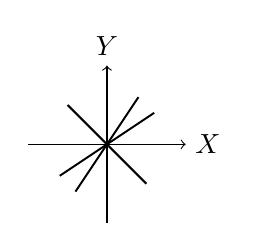
\begin{tikzpicture}
          \draw[->] (-1,0) -- (1,0) node[right] {$X$};
          \draw[->] (0,-1) -- (0,1) node[above] {$Y$};
          \draw[line width=0.25mm] (-0.4,-0.6) -- (0.4,0.6);
          \draw[line width=0.25mm] (-0.6,-0.4) -- (0.6,0.4);
          \draw[line width=0.25mm] (-0.5,0.5) -- (0.5,-0.5);
        \end{tikzpicture}
        \end{center}
\end{lemma}

\begin{proof}
    Induction on $n$. Base case $n = 1$: trivial. \\
    Inductive step: assume $n \geq 2$ and $\bigcup_{i \neq j}V_j \subsetneq V$ for any $j = 1,\cdots,n$. Then there exists $v_j \in V \setminus \{\bigcup_{i \neq j}V_j\}$ for any $j = 1,\cdots,n$. BWOC, suppose $\bigcup_{i=1}^nV_i = V \ni v_j$. Since $v_j \not \in \bigcup_{i \neq j}V_j$, $v_j \in V_j$. Let $1 \leq i \neq j \leq n$. Consider $v_i + \lambda v_j$ with $\lambda \in k$. Check if $\lambda \neq \mu$ in $k$, then $v_i + \lambda v_j \neq v_i + \mu v_j$. So there exists $l$ such that $V_l$ contains two distinct elements $v_i + \lambda v_j$ and $v_i + \mu v_j$ with $\lambda, \mu \neq 0$. Note $V_l \ni (v_i + \lambda v_j) - (v_i + u v_j) = (\lambda - \mu)v_j$. Since $\lambda \neq \mu$, $v_j \in V_l$ and then $l = j$. Note $V_l \ni \lambda^{-1}(v_i + \lambda v_j) - \mu^{-1}(v_i + \mu v_j) = (\lambda^{-1}-\mu^{-1})v_i$. So $v_i \in V_l$ and then $i = l$. Hence $i = l = j$, a contradiction.
\end{proof}

\begin{example}
    If $\abs k < \infty$, then fail. Since $\abs{k^2} < \infty$, $k^2 = \bigcup_{v \in k^2} \{v\} = \bigcup_{0 \neq v \in k^2} \operatorname{span}\{v\}$ finite union but $\operatorname{span}(v) \subsetneq k^2$? \\
    Same technique shows that can's replace $V_1,\cdots,V_n$ with $V_1,V_2,\cdots,$ over $\bbQ$.
\end{example}

\begin{theorem}[More general version]
    Let $\ffb_1,\cdots,\ffb_n \leq R$. Assume
    \begin{enumerate}[(1)]
        \item $R$ contains an infinite field $k$ as a subring, or
        \item $\ffb_3,\cdots,\ffb_n \in \operatorname{Spec}(R)$.
    \end{enumerate}
    Then if $\ffa \subseteq \bigcup_{i=1}^n \ffb_i$, $\ffa \subseteq \ffb_i$ for some $i \in \{1,\cdots,n\}$.
\end{theorem}

\begin{proof}
    \begin{enumerate}[(1)]
        \item Assume $\ffa \not \subseteq \ffb_i$ for any $i = 1,\cdots,n$. Then $\ffa \cap \ffb_i \subsetneq \ffa$ for any $i = 1,\cdots,n$. Since $\ffa$ is a $k$-vector space and $\ffa \cap \ffb_i \lneq \ffa$ for any $i = 1,\cdots,n$, by 1.48, $\ffa \cap \bigcup_{i=1}^n \ffb_i = \bigcup_{i=1}^n (\ffa \cap \ffb_i) \lneq \ffa$. So $\ffa \not \subseteq \bigcup_{i=1}^n \ffb_i$. 
        \item Induct on $n$. Base case $n = 1$: done. Base case $n = 2$. Let $a_i \in \ffa \setminus \ffb_i$ for any $i = 1,2$. Consider $a_1 + a_2 \in \ffa$. Suppose $\ffa \subseteq \ffb_1 \cup \ffb_2$. Then $a_1 + a_2 \in \ffb_1 \cup \ffb_2$, say $a_1 + a_2 \in \ffb_2$. Since $a_1 \in \ffa \subseteq \ffb_1 \cup \ffb_2$ and $a_1 \not \in \ffb_1$, $a_1 \in \ffb_2$. So $a_2 = (a_1 + a_2) - a_1 \in \ffb_2$, a contradiction. \\
            Induct on $n \geq 3$. Assume $\ffa \not \subseteq \ffb_i$ for any $i = 1,\cdots,n$. Suppose $\ffa \subseteq \bigcup_{i=1}^n \ffb_i$. Inducitve hypothesis: $\ffa \not \subseteq \bigcup_{i \neq j} \ffb_i$ for any $j = 1,\cdots,n$, there exists $a_j \in \ffa \setminus \{\bigcup_{i \neq j} \ffb_i\}$. Consider $a_1 \cdot a_{n-1} + a_n \in \ffa \subseteq \bigcup_{i=1}^n \ffb_i$. Since $a_j \in \ffa \subseteq \bigcup_{i=1}^n \ffb_i$ and $a_j \not \in \bigcup_{i \neq j} \ffb_i$, we have $a_j \in V_j$. So there exists $l \in \{1,\cdots,n\}$ such that $a_1 \cdots a_{n-1} + a_n \in \ffb_l$. Suppose $l=n$. Then $a_n \in \ffb_n$ and so $a_1 \cdots a_{n-1} \in \ffb_n$. Since $n \geq 3$, $\ffb_n$ is prime. So $\ffb_n \ni a_i$ for some $i < n$, a contradiction. Hence $l < n$. So $a_1 \cdots a_l \cdots a_{n-1} \in \ffq_l$.
    \end{enumerate}
\end{proof}

\begin{theorem}[Prime Avoidence]
    Let $\ffp_1,\cdots,\ffp_n \in \operatorname{Spec}(R)$. If $\ffa \subseteq \bigcup_{i=1}^n \ffp_i$, then $\ffa \subseteq \ffp_i$ for some $i \in \{1,\cdots,n\}$, i.e., if $\ffa \not \subseteq \ffp_i$ for any $i = 1,\cdots,r$, then $\ffa \not \subseteq \bigcup_{i=1}^n \ffp_i$.
\end{theorem}





\begin{definition}
    Let $\ffa \leq R$ and $S \subseteq R$. $(\ffa:S) = \{r \in R \mid rs \in R,\fa s \in S\}$.
\end{definition}

\begin{example}
    Let $R = k[X,Y]$. $(\langle XY \rangle: \{X,Y\}) = \langle XY \rangle$ and $(\langle X^2,XY \rangle: \{X,Y\}) = \langle X \rangle$.
\end{example}

\begin{fact}
    \begin{enumerate}[(a)]
        \item $\ffa \subseteq (\ffa:S) \leq R$.
        \item $(\ffa:\ffb)\ffb \subseteq \ffa$. 
        \item If $S \subseteq T$, $(\ffa:S) \supseteq (\ffa:T)$.
        \item 
    \end{enumerate}
\end{fact}

\begin{proof}
    \begin{enumerate}
        \item[(b)]
            Let $r \in (\ffa:\ffb)$ and $b \in \ffb$. Then $br \in \ffa$. So all generators of $(\ffa:\ffb)\ffb$ is in $\ffa$.
        \item[(e)]
            Since $S \subseteq \langle S \rangle$, by (c), $(\ffa:S) \supseteq (\ffa:\langle S \rangle)$. ``$\subseteq$''.
        \item [(j)]
            ``$\subseteq$''.\\
            ``$\supseteq$''. Reverse the above proof.
    \end{enumerate}
\end{proof}

\begin{example}
    Let $R = k[X,Y]$.
\end{example}

\begin{definition}
    The \emph{radical} of $\ffa \leq R$ is $\operatorname{rad}(\ffa) = \operatorname{r}(\ffa) = \sqrt \ffa = \{x \in R \mid x^n \in \ffa, \fa n \geq\geq 0\} = \{x \in R \mid x^n \in \ffa \text{ for some }n \in \bbN\}$. 
\end{definition}

\begin{example}
    $\operatorname{rad}(\langle X^2Y,XY^2 \rangle) = \langle XY \rangle$ in $k[X,Y]$.
\end{example}
